\subsection{Caso 1. TCP SYN Flood: indisponibilidad y agotamiento de conexiones}
\label{caso:syn-flood}

\begin{situacion}
Un servidor web de laboratorio responde lentamente o deja de aceptar nuevas conexiones.
\textbf{Objetivo:} \par
Analizar el comportamiento del establecimiento de conexiones TCP para identificar posibles indicadores de un ataque SYN Flood, mediante la inspección de paquetes de red, el análisis de conexiones y la revisión de registros del sistema.

Se busca identificar patrones anormales en las solicitudes SYN, respuestas SYN/ACK y confirmaciones ACK, así como proponer mecanismos de detección y mitigación que contribuyan a proteger la disponibilidad de los servicios de red. \par
\textbf{Fundamento Teórico:} \par
TCP (Transmission Control Protocol) es un protocolo de transporte orientado a conexión que utiliza un proceso de establecimiento conocido como Three-Way Handshake.\par
Este proceso consta de tres etapas:
\begin{itemize}
	\item SYN: el cliente solicita establecer una conexión.
	\item SYN/ACK: el servidor responde aceptando la solicitud.
	\item ACK: el cliente confirma la respuesta y se completa el establecimiento de la conexión.
\end{itemize}
Un ataque SYN Flood busca agotar los recursos del servidor mediante el envío de numerosas solicitudes SYN que pueden quedar sin completar. Esto puede provocar una acumulación de conexiones pendientes y afectar la disponibilidad del servicio.
\end{situacion}

\paragraph{Procedimiento:} 
El análisis forense y de tráfico se llevó a cabo siguiendo una serie de pasos secuenciales respaldados por las evidencias capturadas:

\begin{enumerate}
    \item \textbf{Preparación y verificación de la captura PCAP:} \par Se verificó la integridad del archivo de captura utilizado mediante el cálculo de su huella criptográfica SHA-256 en entorno PowerShell, obteniendo el valor hash correspondiente al archivo analizado, como se observa en la Figura~\ref{fig:01_hash_original}.
    \item \textbf{Identificación de paquetes SYN mediante Wireshark:} \par Se cargó el archivo \texttt{200722\_tcp\_anon.pcapng} en la herramienta Wireshark y se aplicó el filtro de visualización \texttt{tcp.flags.syn == 1 \&\& tcp.flags.ack == 0} para aislar las solicitudes de inicio de conexión puras (paquetes SYN), identificando las tramas correspondientes (Figura~\ref{fig:02_paquetes_SYN}).
    \item \textbf{Identificación de respuestas SYN/ACK:} \par Se aplicó el filtro \texttt{tcp.flags.syn == 1 \&\& tcp.flags.ack == 1} para localizar las respuestas del servidor aceptando las conexiones solicitadas (Figura~\ref{fig:03_paquetes_SYN_ACK}).
    \item \textbf{Inspección del establecimiento de conexiones y Handshake:} \par Mediante el filtro \texttt{tcp.flags.ack == 1 \&\& tcp.flags.syn == 0}, se examinaron los paquetes de confirmación ACK y el flujo posterior de la comunicación, incluyendo intercambio de datos y cierre de sesión (Figura~\ref{fig:04_handshake_TCP}).
    \item \textbf{Inspección de conversaciones TCP:} \par Se utilizó la herramienta de estadísticas de conversaciones TCP de Wireshark para analizar los flujos de comunicación entre las direcciones IP involucradas (Figura~\ref{fig:05_statics_tcp}).
    \item \textbf{Análisis temporal de solicitudes y respuestas:} \par Se emplearon las gráficas de E/S (\textit{I/O Graphs}) de Wireshark configurando filtros específicos para tramas SYN (Figura~\ref{fig:06_Statics_IO_SYNC}) y SYN/ACK (Figura~\ref{fig:07_Statics_SYNC-ACK}) con el fin de evaluar la distribución temporal del tráfico.
    \item \textbf{Inspección de conexiones TCP locales:} \par Se revisó el estado de las conexiones de red del sistema mediante comandos de diagnóstico para evaluar los estados actuales de los sockets (Figura~\ref{fig:08_conexiones_netstat}).
\end{enumerate}

\begin{figure}[htbp]
    \centering
    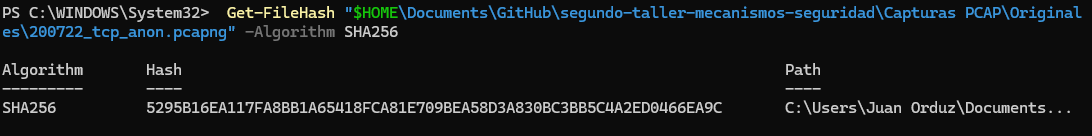
\includegraphics[width=0.95\textwidth]{imagenes/Evidencias CU-1/01_hash_original.png}
    \caption{Verificación de integridad del archivo PCAP mediante el cálculo de hash SHA-256.}
    \label{fig:01_hash_original}
\end{figure}

\begin{figure}[htbp]
    \centering
    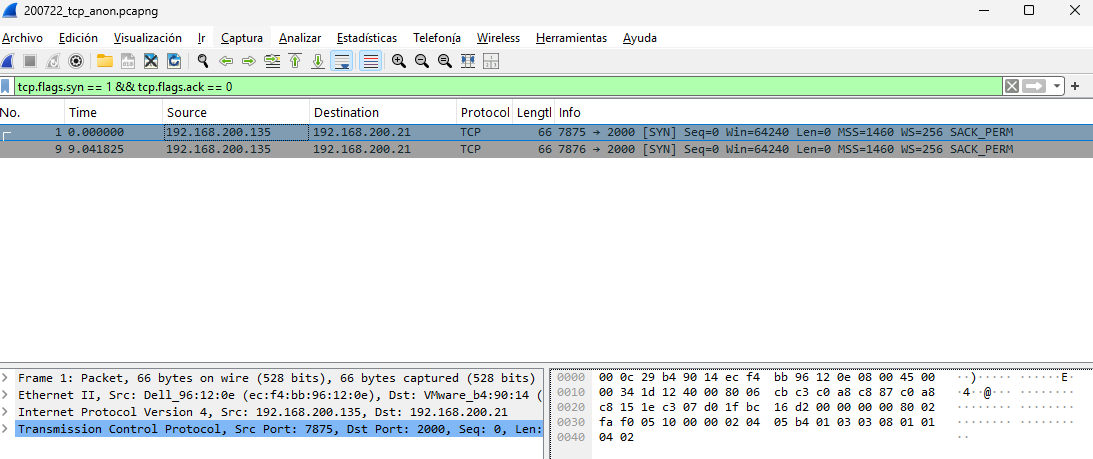
\includegraphics[width=0.95\textwidth]{imagenes/Evidencias CU-1/02_paquetes_SYN.png}
    \caption{Filtrado de solicitudes de inicio de conexión SYN (\texttt{tcp.flags.syn == 1 \&\& tcp.flags.ack == 0}) en Wireshark.}
    \label{fig:02_paquetes_SYN}
\end{figure}

\begin{figure}[htbp]
    \centering
    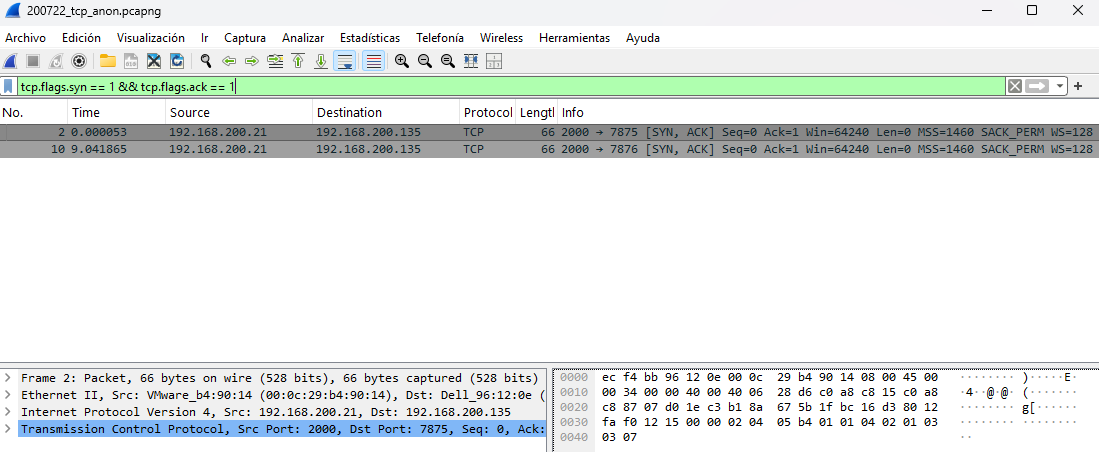
\includegraphics[width=0.95\textwidth]{imagenes/Evidencias CU-1/03_paquetes_SYN_ACK.png}
    \caption{Identificación de respuestas SYN/ACK del servidor (\texttt{tcp.flags.syn == 1 \&\& tcp.flags.ack == 1}).}
    \label{fig:03_paquetes_SYN_ACK}
\end{figure}

\begin{figure}[htbp]
    \centering
    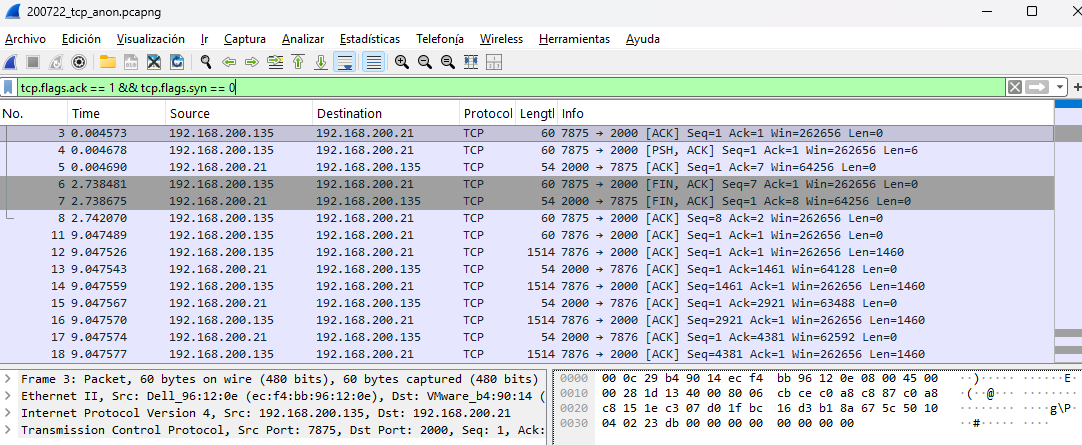
\includegraphics[width=0.95\textwidth]{imagenes/Evidencias CU-1/04_handshake_TCP.png}
    \caption{Inspección de paquetes ACK y tráfico posterior de la sesión TCP.}
    \label{fig:04_handshake_TCP}
\end{figure}

\begin{figure}[htbp]
    \centering
    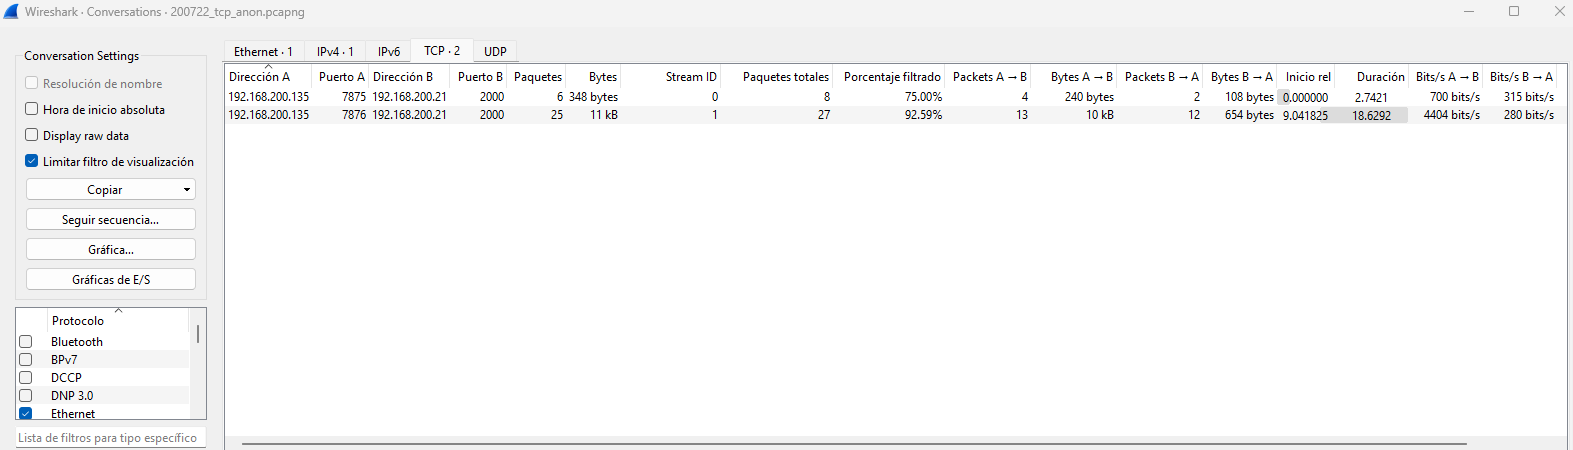
\includegraphics[width=0.95\textwidth]{imagenes/Evidencias CU-1/05_statics_tcp.png}
    \caption{Estadísticas de conversaciones TCP recopiladas en Wireshark.}
    \label{fig:05_statics_tcp}
\end{figure}

\begin{figure}[htbp]
    \centering
    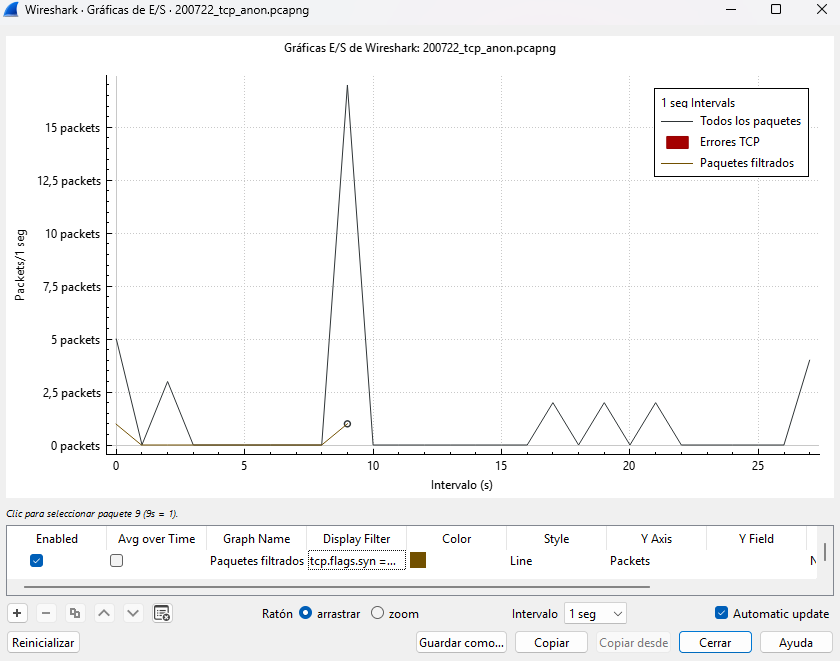
\includegraphics[width=0.95\textwidth]{imagenes/Evidencias CU-1/06_Statics_IO_SYNC.png}
    \caption{Gráfica de E/S de Wireshark para el análisis temporal de paquetes SYN filtrados.}
    \label{fig:06_Statics_IO_SYNC}
\end{figure}

\begin{figure}[htbp]
    \centering
    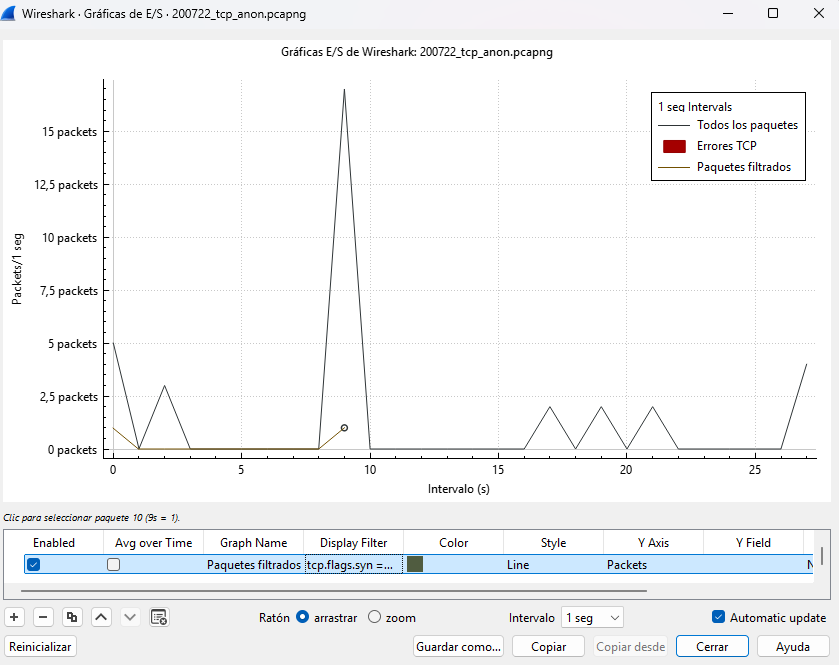
\includegraphics[width=0.95\textwidth]{imagenes/Evidencias CU-1/07_Statics_SYNC-ACK.png}
    \caption{Gráfica de E/S de Wireshark para el análisis temporal de respuestas SYN/ACK.}
    \label{fig:07_Statics_SYNC-ACK}
\end{figure}

\begin{figure}[htbp]
    \centering
    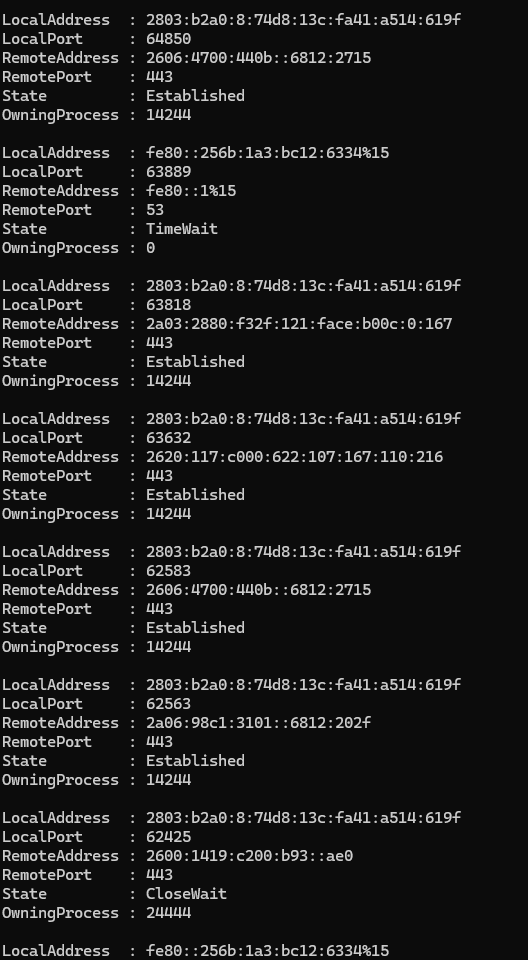
\includegraphics[width=0.75\textwidth]{imagenes/Evidencias CU-1/08_conexiones_netstat.png}
    \caption{Inspección de estados de conexiones de red locales mediante comandos de diagnóstico.}
    \label{fig:08_conexiones_netstat}
\end{figure}

\paragraph{Resultados obtenidos:}
A partir de la inspección de las evidencias proporcionadas por las capturas de Wireshark y las herramientas del sistema, se extrajeron los siguientes resultados cuantitativos y cualitativos:

\begin{itemize}
    \item \textbf{Análisis de paquetes SYN y SYN/ACK:} En las capturas de Wireshark se identificaron explícitamente dos solicitudes SYN principales (tramas 1 y 9) originadas desde la dirección IP \texttt{192.168.200.135} (puertos \texttt{7875} y \texttt{7876}) dirigidas al servidor \texttt{192.168.200.21} en el puerto \texttt{2000} (Figura~\ref{fig:02_paquetes_SYN}). Asimismo, el servidor respondió simétricamente con dos paquetes SYN/ACK (tramas 2 y 10) hacia los mismos puertos de origen (Figura~\ref{fig:03_paquetes_SYN_ACK}).
    \item \textbf{Conversaciones TCP:} Las estadísticas de conversaciones TCP (Figura~\ref{fig:05_statics_tcp}) reflejan los flujos de comunicación identificados en la captura:
\end{itemize}

\begin{table}[htbp]
    \centering
    \caption{Tabla de conversaciones TCP extraídas de la evidencia.}
    \label{tab:conversaciones_tcp}
    \begin{tabular}{cccccccc}
        \toprule
        \textbf{IP Origen} & \textbf{Puerto A} & \textbf{IP Destino} & \textbf{Puerto B} & \textbf{Paquetes Totales} & \textbf{Bytes Totales} & \textbf{Duración (s)} \\
        \midrule
        192.168.200.135 & 7875 & 192.168.200.21 & 2000 & 8 & 348 bytes & 2.7421 \\
        192.168.200.135 & 7876 & 192.168.200.21 & 2000 & 27 & 11 kB & 18.6292 \\
        \bottomrule>
    \end{tabular}
\end{table}

\begin{itemize}
    \item \textbf{Estados de conexión locales:} La inspección mediante comandos de red (Figura~\ref{fig:08_conexiones_netstat}) muestra múltiples conexiones activas asociadas a procesos del sistema, reportando predominantemente estados como \texttt{Established}, además de estados de cierre y espera como \texttt{TimeWait} y \texttt{CloseWait}, con identificadores de proceso (\texttt{OwningProcess}) numéricos específicos (ej. \texttt{14244} y \texttt{24444}).
\end{itemize}

\paragraph{Análisis de resultados:}
Al contrastar las evidencias obtenidas, se observa un comportamiento normal y completado del \textit{Three-Way Handshake} para las conexiones analizadas. Cada paquete SYN enviado por el cliente (\texttt{192.168.200.135}) obtuvo una respuesta SYN/ACK correspondiente por parte del servidor (\texttt{192.168.200.21}), seguida de los paquetes ACK correspondientes que permitieron establecer la comunicación y realizar transferencia de datos (como se visualiza en las tramas de la Figura~\ref{fig:04_handshake_TCP} y las duraciones registradas en la Tabla~\ref{tab:conversaciones_tcp}). \newline

Si bien las gráficas temporales de E/S (Figuras~\ref{fig:06_Statics_IO_SYNC} y \ref{fig:07_Statics_SYNC-ACK}) muestran un pico puntual de tráfico que alcanza aproximadamente 17 paquetes por segundo en el intervalo de los 9 segundos, este incremento responde a una ráfaga legítima de intercambio de datos y cierre de conexiones, y no a una acumulación masiva de solicitudes SYN huérfanas. \newline
\paragraph{Limitaciones de las evidencias:} Las trazas analizadas corresponden a un escenario de tráfico controlado con un volumen reducido de transacciones entre IPs específicas; por lo tanto, las evidencias no muestran síntomas de saturación, agotamiento de recursos ni un ataque SYN Flood activo.

\paragraph{Indicadores de detección:}
A partir del análisis de las evidencias, se evalúan los siguientes indicadores de seguridad:
\begin{itemize}
    \item \textbf{Picos de solicitudes SYN:} Observado puntualmente en la gráfica temporal (Figura~\ref{fig:06_Statics_IO_SYNC}), pero asociado a tráfico legítimo.
    \item \textbf{Solicitudes SYN sin completar el handshake:} No observado; todas las solicitudes contaron con su respectiva respuesta y confirmación.
    \item \textbf{Incremento de conexiones pendientes:} No verificado en las capturas analizadas.
    \item \textbf{Múltiples fuentes generando solicitudes:} No observado, el tráfico proviene de una única IP cliente (\texttt{192.168.200.135}).
    \item \textbf{Comportamiento temporal inusual:} Se detectó un pico temporal aislado a los 9 segundos, el cual fue verificado como parte de la transferencia normal de la sesión (Figura~\ref{fig:05_statics_tcp}).
\end{itemize}

\paragraph{Regla de detección propuesta:}
Para la identificación temprana de anomalías de tipo SYN Flood en entornos de producción, se propone una regla conceptual basada en umbrales dinámicos respecto a la línea base del servicio:
\begin{equation*}
    \text{Alerta SYN Flood} \iff \left( \frac{\text{Conteo SYN}_{\Delta t}}{\text{Conteo SYN/ACK}_{\Delta t}} > \alpha \right) \land \left( \text{Conexiones}_{\text{Half-Open}} > \text{Umbral}_{\text{baseline}} \right)
\end{equation*}
Donde $\alpha$ representa el factor de proporción esperado entre solicitudes de establecimiento y respuestas del servidor, y los umbrales numéricos deben calibrarse estrictamente de acuerdo con el comportamiento histórico y la capacidad de procesamiento del servicio protegido. \newline

\paragraph{Mitigación y defensa}
Para garantizar la resiliencia de la infraestructura ante posibles escenarios de denegación de servicio por agotamiento de conexiones, se recomiendan las siguientes medidas técnicas:
\begin{itemize}
    \item \textbf{Actualización de sistemas:} Mantener actualizados el sistema operativo y los servicios expuestos para parchear vulnerabilidades de pila de red.
    \item \textbf{Limitación de exposición:} Reducir la superficie de ataque limitando el acceso a los servicios únicamente a redes o segmentos autorizados.
    \item \textbf{Mecanismos de protección nativos:} Habilitar tecnologías de mitigación a nivel de sistema operativo como \textit{SYN Cookies} para evitar el consumo de memoria en la cola de conexiones pendientes (\textit{backlog}).
    \item \textbf{Control de tasa (\textit{Rate Limiting}):} Aplicar políticas de control de tráfico en los dispositivos de borde o cortafuegos para limitar ráfagas excesivas de solicitudes SYN.
    \item \textbf{Monitorización continua:} Vigilar activamente el estado de las colas de conexiones y escalar incidentes al equipo de infraestructura ante anomalías sostenidas.
\end{itemize}
Es indispensable validar que la implementación de estas medidas no restrinja ni bloquee el acceso a los clientes legítimos de la red.

\paragraph{Preguntas de análisis}
\begin{enumerate}
    \item \textbf{¿Qué recursos mantiene el servidor durante el handshake TCP?}\par
    Durante el proceso de establecimiento de conexión (\textit{Three-Way Handshake}), el servidor web reserva recursos críticos en su pila de red. Al recibir una solicitud SYN, el núcleo del sistema operativo asigna una entrada en la cola de conexiones pendientes (\textit{SYN backlog queue}) y crea una estructura de control de socket (\textit{Transmission Control Block - TCB}), consumiendo memoria RAM y ciclos de procesamiento para gestionar los temporizadores de retransmisión y los números de secuencia iniciales hasta recibir la confirmación ACK final.
    \item \textbf{¿Qué falsos positivos pueden producir picos legítimos?}\par
    Un incremento repentino en la tasa de solicitudes SYN no siempre denota actividad maliciosa. Entre los factores legítimos que pueden generar picos temporales se encuentran: la concurrencia masiva de usuarios en horarios pico, el inicio simultáneo de aplicaciones cliente, reintentos automáticos de conexión ante intermitencias temporales de la red, la ejecución de actualizaciones de software o la apertura múltiple de conexiones persistentes de tipo HTTP/2 o HTTP/3 por parte de navegadores modernos.
\end{enumerate}

\paragraph{Conclusiones:}
\begin{itemize}
    \item Se logró analizar exitosamente el contenido del archivo de captura PCAP mediante la verificación de su integridad criptográfica y la inspección detallada de tramas en Wireshark.
    \item Se identificó un comportamiento TCP completamente normal y estructurado mediante el \textit{Three-Way Handshake}, donde las solicitudes SYN enviadas por la IP \texttt{192.168.200.135} obtuvieron respuestas SYN/ACK y confirmaciones ACK válidas por parte del servidor \texttt{192.168.200.21}.
    \item No fue posible comprobar la existencia de indicadores de un ataque SYN Flood debido a que el volumen de tráfico analizado es reducido y no presenta conexiones huérfanas ni desproporción entre solicitudes y respuestas.
    \item El análisis presentó limitaciones derivadas de la naturaleza acotada de la muestra de tráfico de laboratorio, la cual carece de escala masiva.
    \item Se determinó la pertinencia de implementar mecanismos defensivos preventivos, tales como \textit{SYN Cookies} y políticas de control de tasa, para proteger la disponibilidad futura ante eventuales contingencias de denegación de servicio.
\end{itemize}

\begin{table}[H]
    \centering
    \caption{Ficha de registro del hallazgo. Caso 1}
    \footnotesize
    \renewcommand{\arraystretch}{1.2}
    \begin{tabularx}{\textwidth}{@{}>{\raggedright\arraybackslash}p{0.23\textwidth} Y@{}}
        \toprule
        \textbf{Campo} & \textbf{Registro} \\
        \midrule
        Identificador & Caso 1 (TCP SYN Flood), Evidencias 01 a 08 (\texttt{01\_hash\_original.png} a \texttt{08\_conexiones\_netstat.png}). Analista: Juan David Orduz. \\ \hline
        Fecha y hora & Captura analizada: \texttt{200722\_tcp\_anon.pcapng} (datos anonimizados del 20 de julio de 2007). \\ \hline
        Origen/destino & Tráfico observado entre el cliente \texttt{192.168.200.135} (puertos \texttt{7875}, \texttt{7876}) y el servidor \texttt{192.168.200.21} (puerto \texttt{2000}). \\ \hline
        Observación & Análisis forense de tráfico de red en Wireshark y revisión de conexiones locales mediante consola. Se identificó un establecimiento de conexión TCP normal (\textit{Three-Way Handshake}) sin evidencias de ataque SYN Flood. \\ \hline
        Hipótesis & Si el servidor experimenta un ataque SYN Flood, se observará una desproporción masiva de paquetes SYN frente a SYN/ACK y una acumulación de conexiones semiconectadas (\textit{half-open}). \\ \hline
        Validación & Las capturas y estadísticas de Wireshark (Figuras~\ref{fig:02_paquetes_SYN} a \ref{fig:07_Statics_SYNC-ACK}) y de red (Figura~\ref{fig:08_conexiones_netstat}) mostraron simetría total en el \textit{handshake}, descartando anomalías de denegación de servicio. \\ \hline
        Severidad & Baja / Informativa (Escenario de laboratorio con tráfico nominal controlado). \\ \hline
        Acción & Documentar los resultados técnicos reales, descartar la hipótesis de ataque por falta de indicadores y proponer directrices de monitorización preventiva y mitigación. \\ \hline
        Integridad & Archivo de captura validado mediante huella criptográfica SHA-256 (\texttt{5295B16EA117FA8BB1A65418FCA81E709BEA58D3A830BC3BB5C4A2ED0466EA9C}). \\
        \bottomrule
    \end{tabularx}
\end{table}